\section{Auswertung}
\label{sec:Auswertung}


\subsubsection{(a) Erzeugen einer amplitudenmodulierten Schwingung mit
Hilfe eines Ringmodulators}
\label{subsubsec:auswertung_a}
In der Abbildung \ref{fig:ringamp_zeit} ist das Modulationssignal
sowie die amplitudenmodulierte Schwingung, die mit einem Ringmodulatorschaltung \ref{fig:5}
erzeugt wird,
in Abhänigkeit der Zeit dargestellt.
Die Modulationsfrequenz beträgt $\SI{100(5)}{\kilo\hertz}$
und die Trägerfrequenz $\SI{1.00(5)}{\mega\hertz}$.
\begin{figure}
  \centering
  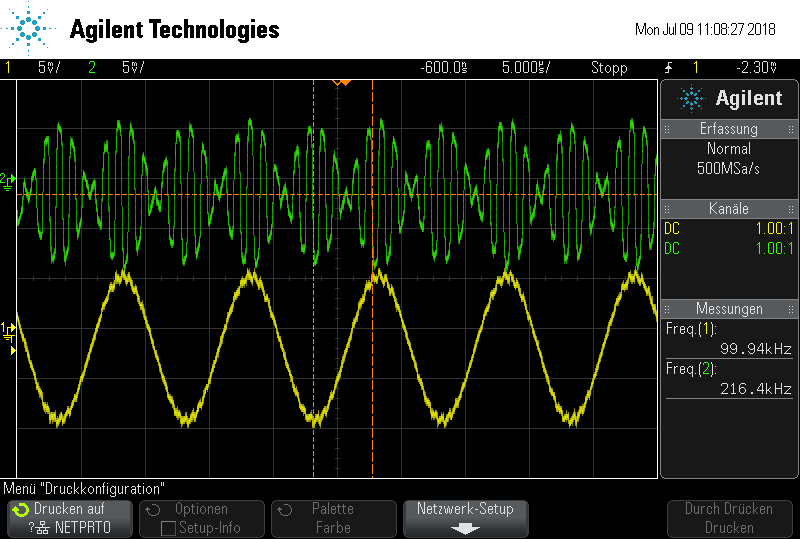
\includegraphics[width=0.7\textwidth]{osci/amp_ringmodulator.png}
  \caption{Amplitudenmodulierte
  Schwingung eines Ringmodulators und das entsprechende Modulationssignal.}
  \label{fig:ringamp_zeit}
\end{figure}


\subsubsection{(b) Untersuchung des Frequenzspektrums einer
amplitudenmodulierten Schwingung}
\label{subsubsec:auswertung_b}

Die aus Kapitel \ref{subsubsec:auswertung_a} erzeugete
amplitudenmodulierte Schwingung wird in Abbildung \ref{fig:ringamp_frequenz}
im Frequenzraum dargestellt.
\begin{figure}
  \centering
  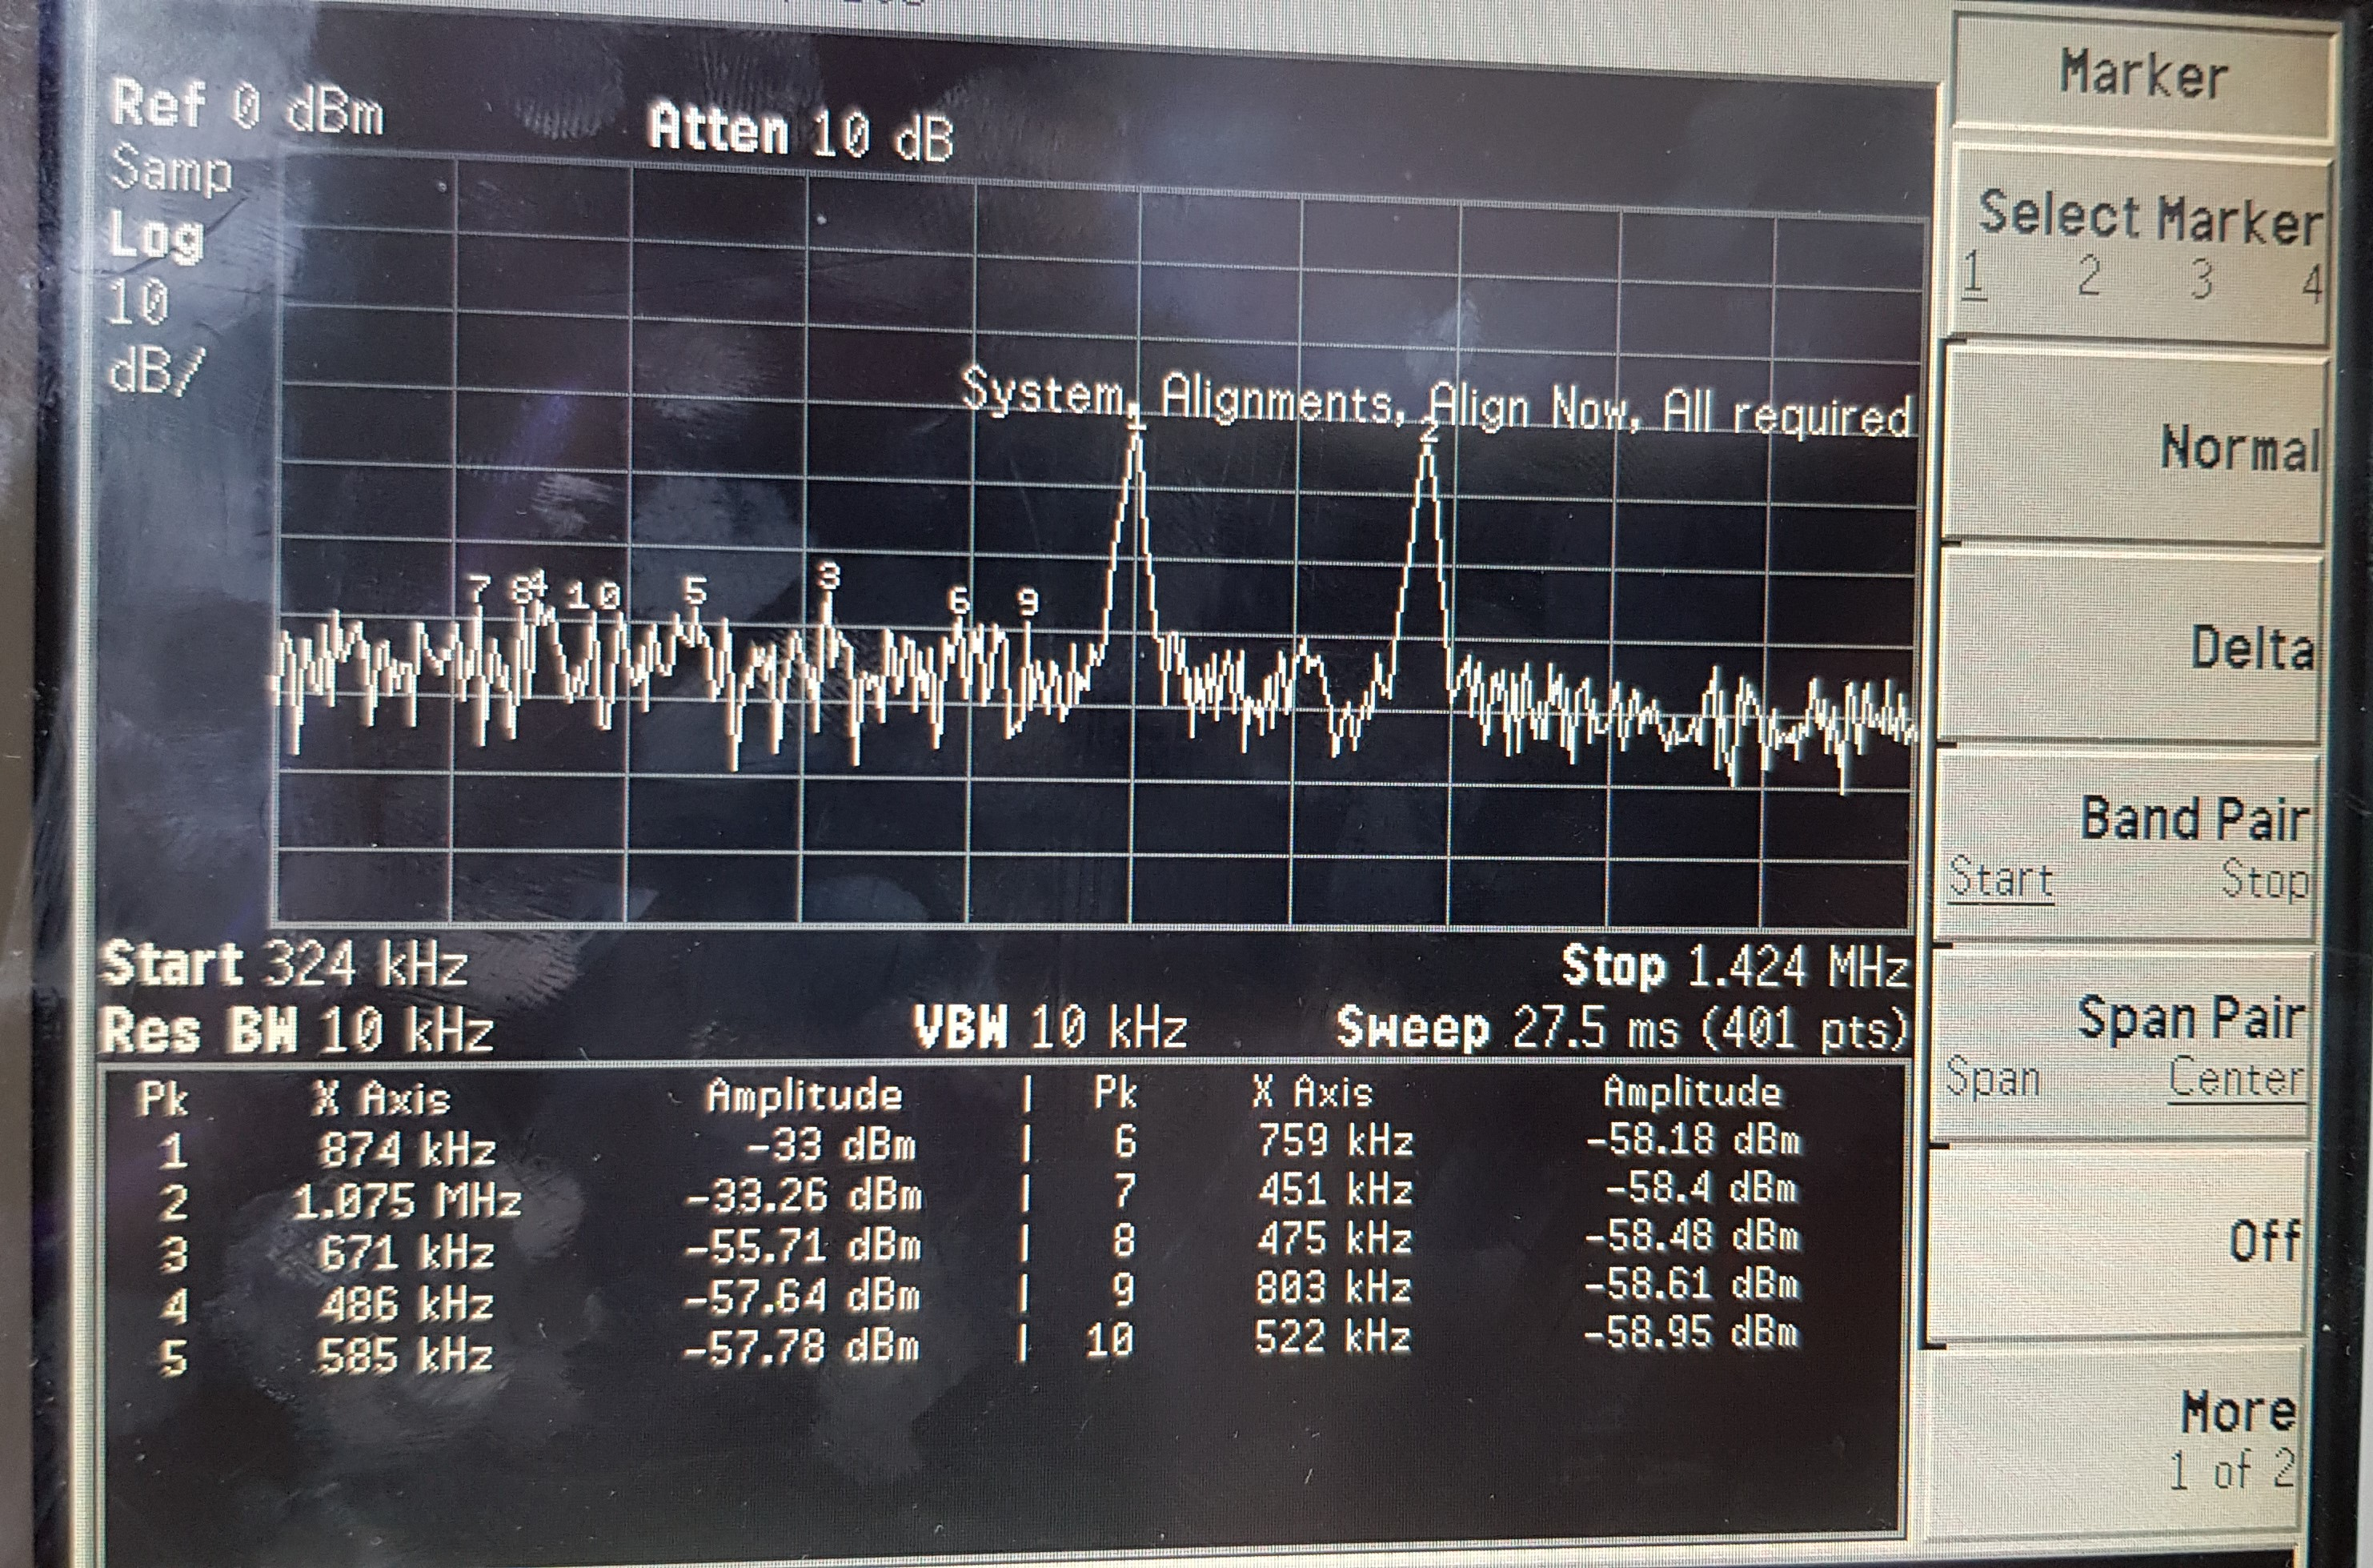
\includegraphics[width=0.7\textwidth]{spec/frequenzbereich_klein_ring.jpg}
  \caption{Amplitudenmodulierte
  Schwingung eines Ringmodulators im Frequenzraum.}
  \label{fig:ringamp_frequenz}
\end{figure}
Aus der Abbildung \ref{fig:ringamp_frequenz}
können die beiden aus der Modulation resultierenden Frequenzen
\begin{align}
  f_{\text{T}}+f_{\text{M}}=\SI{0.87(5)}{\mega\hertz}
  f_{\text{T}}-f_{\text{M}}=\SI{1.07(5)}{\mega\hertz}
\end{align}
bestimmt werden.
Deutlich wird ebendfalls das es keine Trägerabstrahlung vorliegt und
keine Terme höherer Ordnung auftreten.

\subsubsection{(c) Erzeugen einer amplitudenmodulierten Schwingung
mit Hilfe einer Gleichrichterdiode}
\label{subsubsec:auswertung_c}
Anstelle des Ringmodulator wird eine Diode wie in Schaltung \ref{fig:14} zur Amplitudenmodulation verwendnet.
Die Abbildungen \ref{fig:diode_zeit} und \ref{fig:diode_frequenz_klein}
enthälten
sowohl das zeitabhänige Signal und das Signal im Frequenzraum.
Als Frequenzen werden $f_{\text{T}}=\SI{2.50(5)}{\mega\hertz}$ und
$f_{\text{M}}=\SI{0.10(1)}{\mega\hertz}$ verwendet.
\begin{figure}
  \centering
  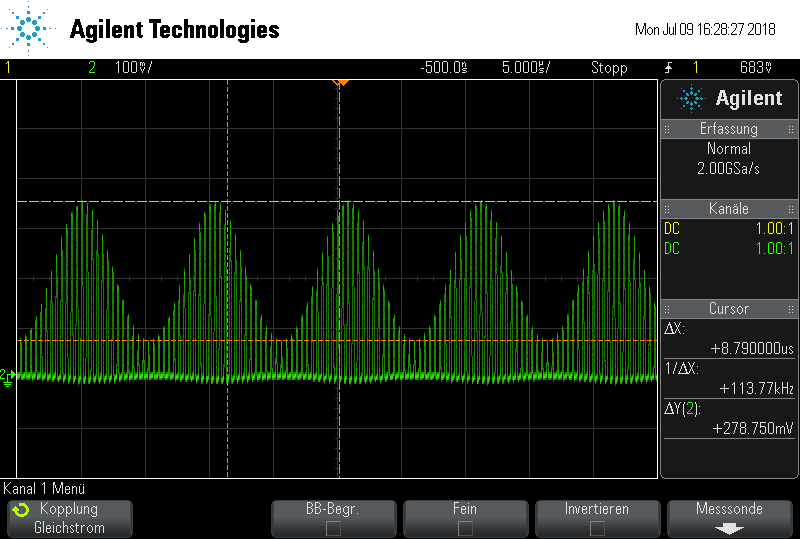
\includegraphics[width=0.7\textwidth]{osci/amp_mod_diode.png}
  \caption{Amplitudenmodulierte
  Schwingung einer Diode nach dem Aufbau aus Abb.\ref{fig:14}.}
  \label{fig:diode_zeit}
\end{figure}

Aus Abbildung \ref{fig:diode_zeit} folgt der Abstand $\Delta U$ zwischen dem maximum und minimum Einhüllenden
\begin{align}
  \Delta U &= U_{\text{T}}(1+m)-U_{\text{T}}(1-m) =2*U_{\text{T}} = \SI{0.27(2)}{\volt}
\intertext{und somit für den Modulationsgrad}
    m &= ?? .
\end{align}

\begin{figure}
  \centering
  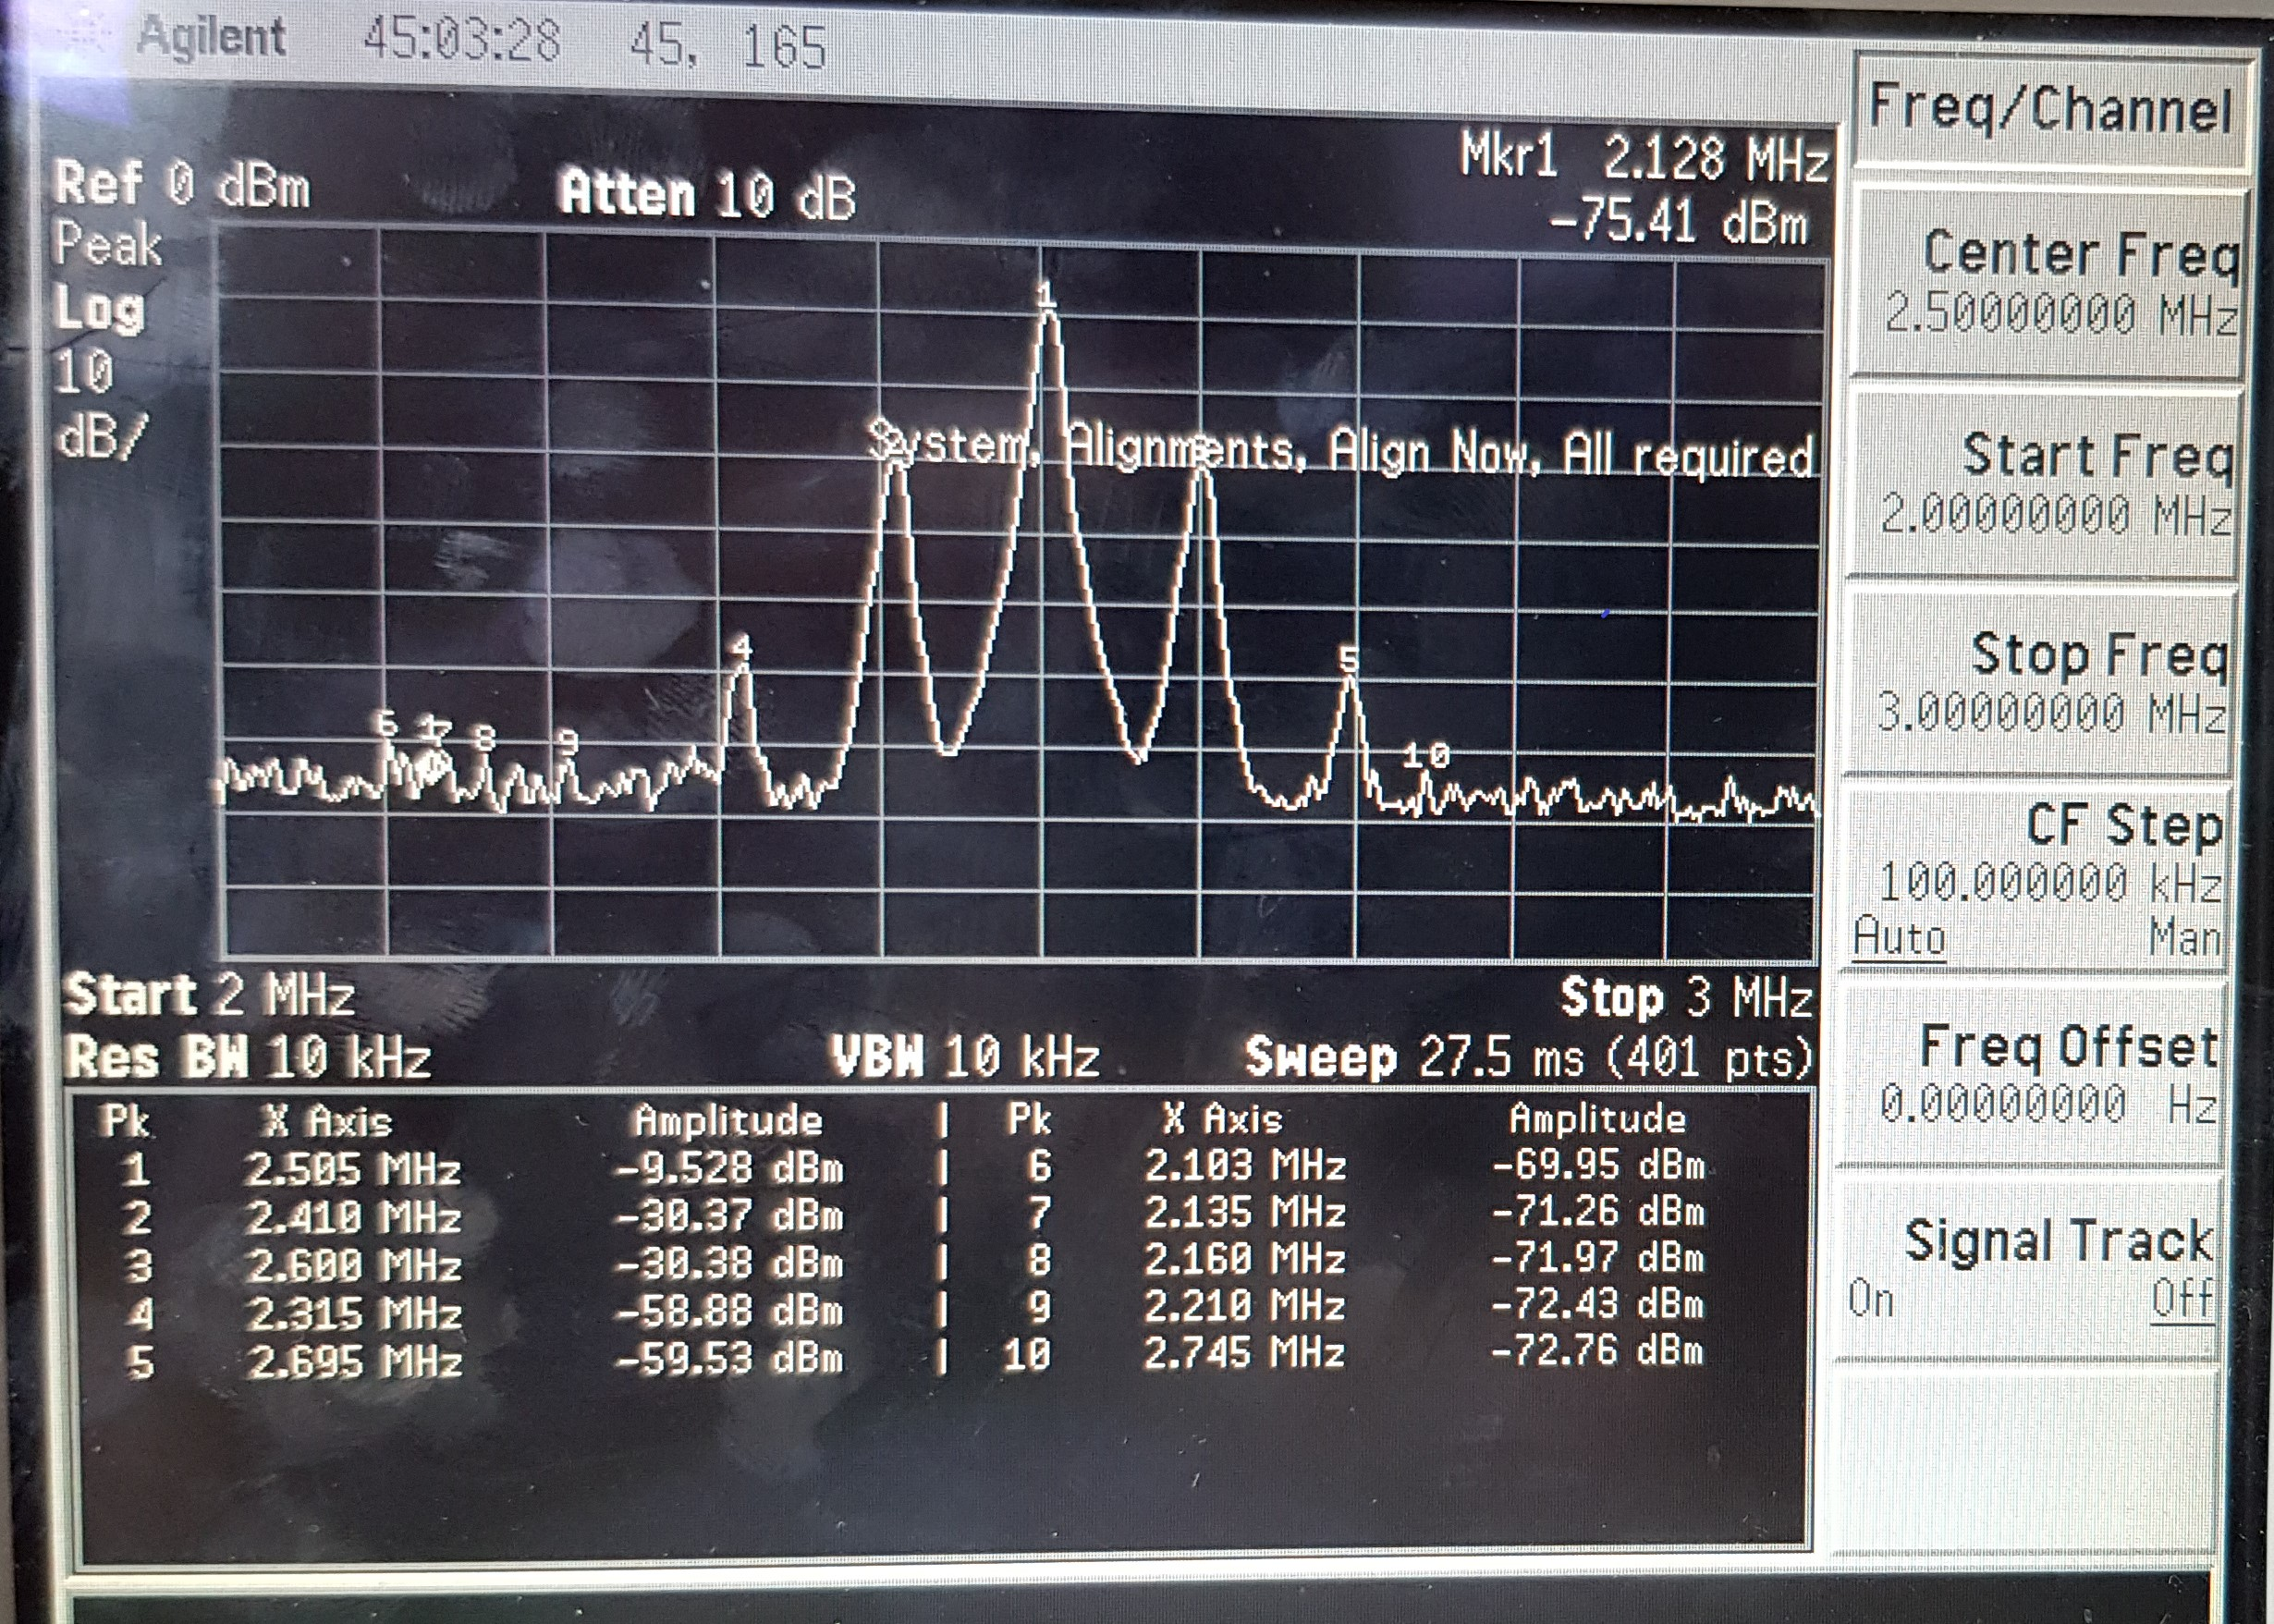
\includegraphics[width=0.7\textwidth]{spec/frequenzbereich_klein_diode.jpg}
  \caption{Amplitudenmodulierte
Schwingung einer Diode im Frequenzraum.}
  \label{fig:diode_frequenz_klein}
\end{figure}
Aus der Abbildung \ref{fig:diode_frequenz_klein}
wird die Trägerabstrahlung
sowie
die auftetenden Mischterme durch die nicht linerare
Kennlinie
der Diode deutlich.
Die Abbildung \ref{fig:diode_frequenz_gross}
für einene größeren Frequenzbereich
verdeutlich dies ebenfalls, da Terme bis
zu $\mathcal{O}\left(U^4\right)$
also Frequenzen mit beispielsweise $4U_{\text{T}}$
deutlich sichtbar sind.
\begin{figure}
  \centering
  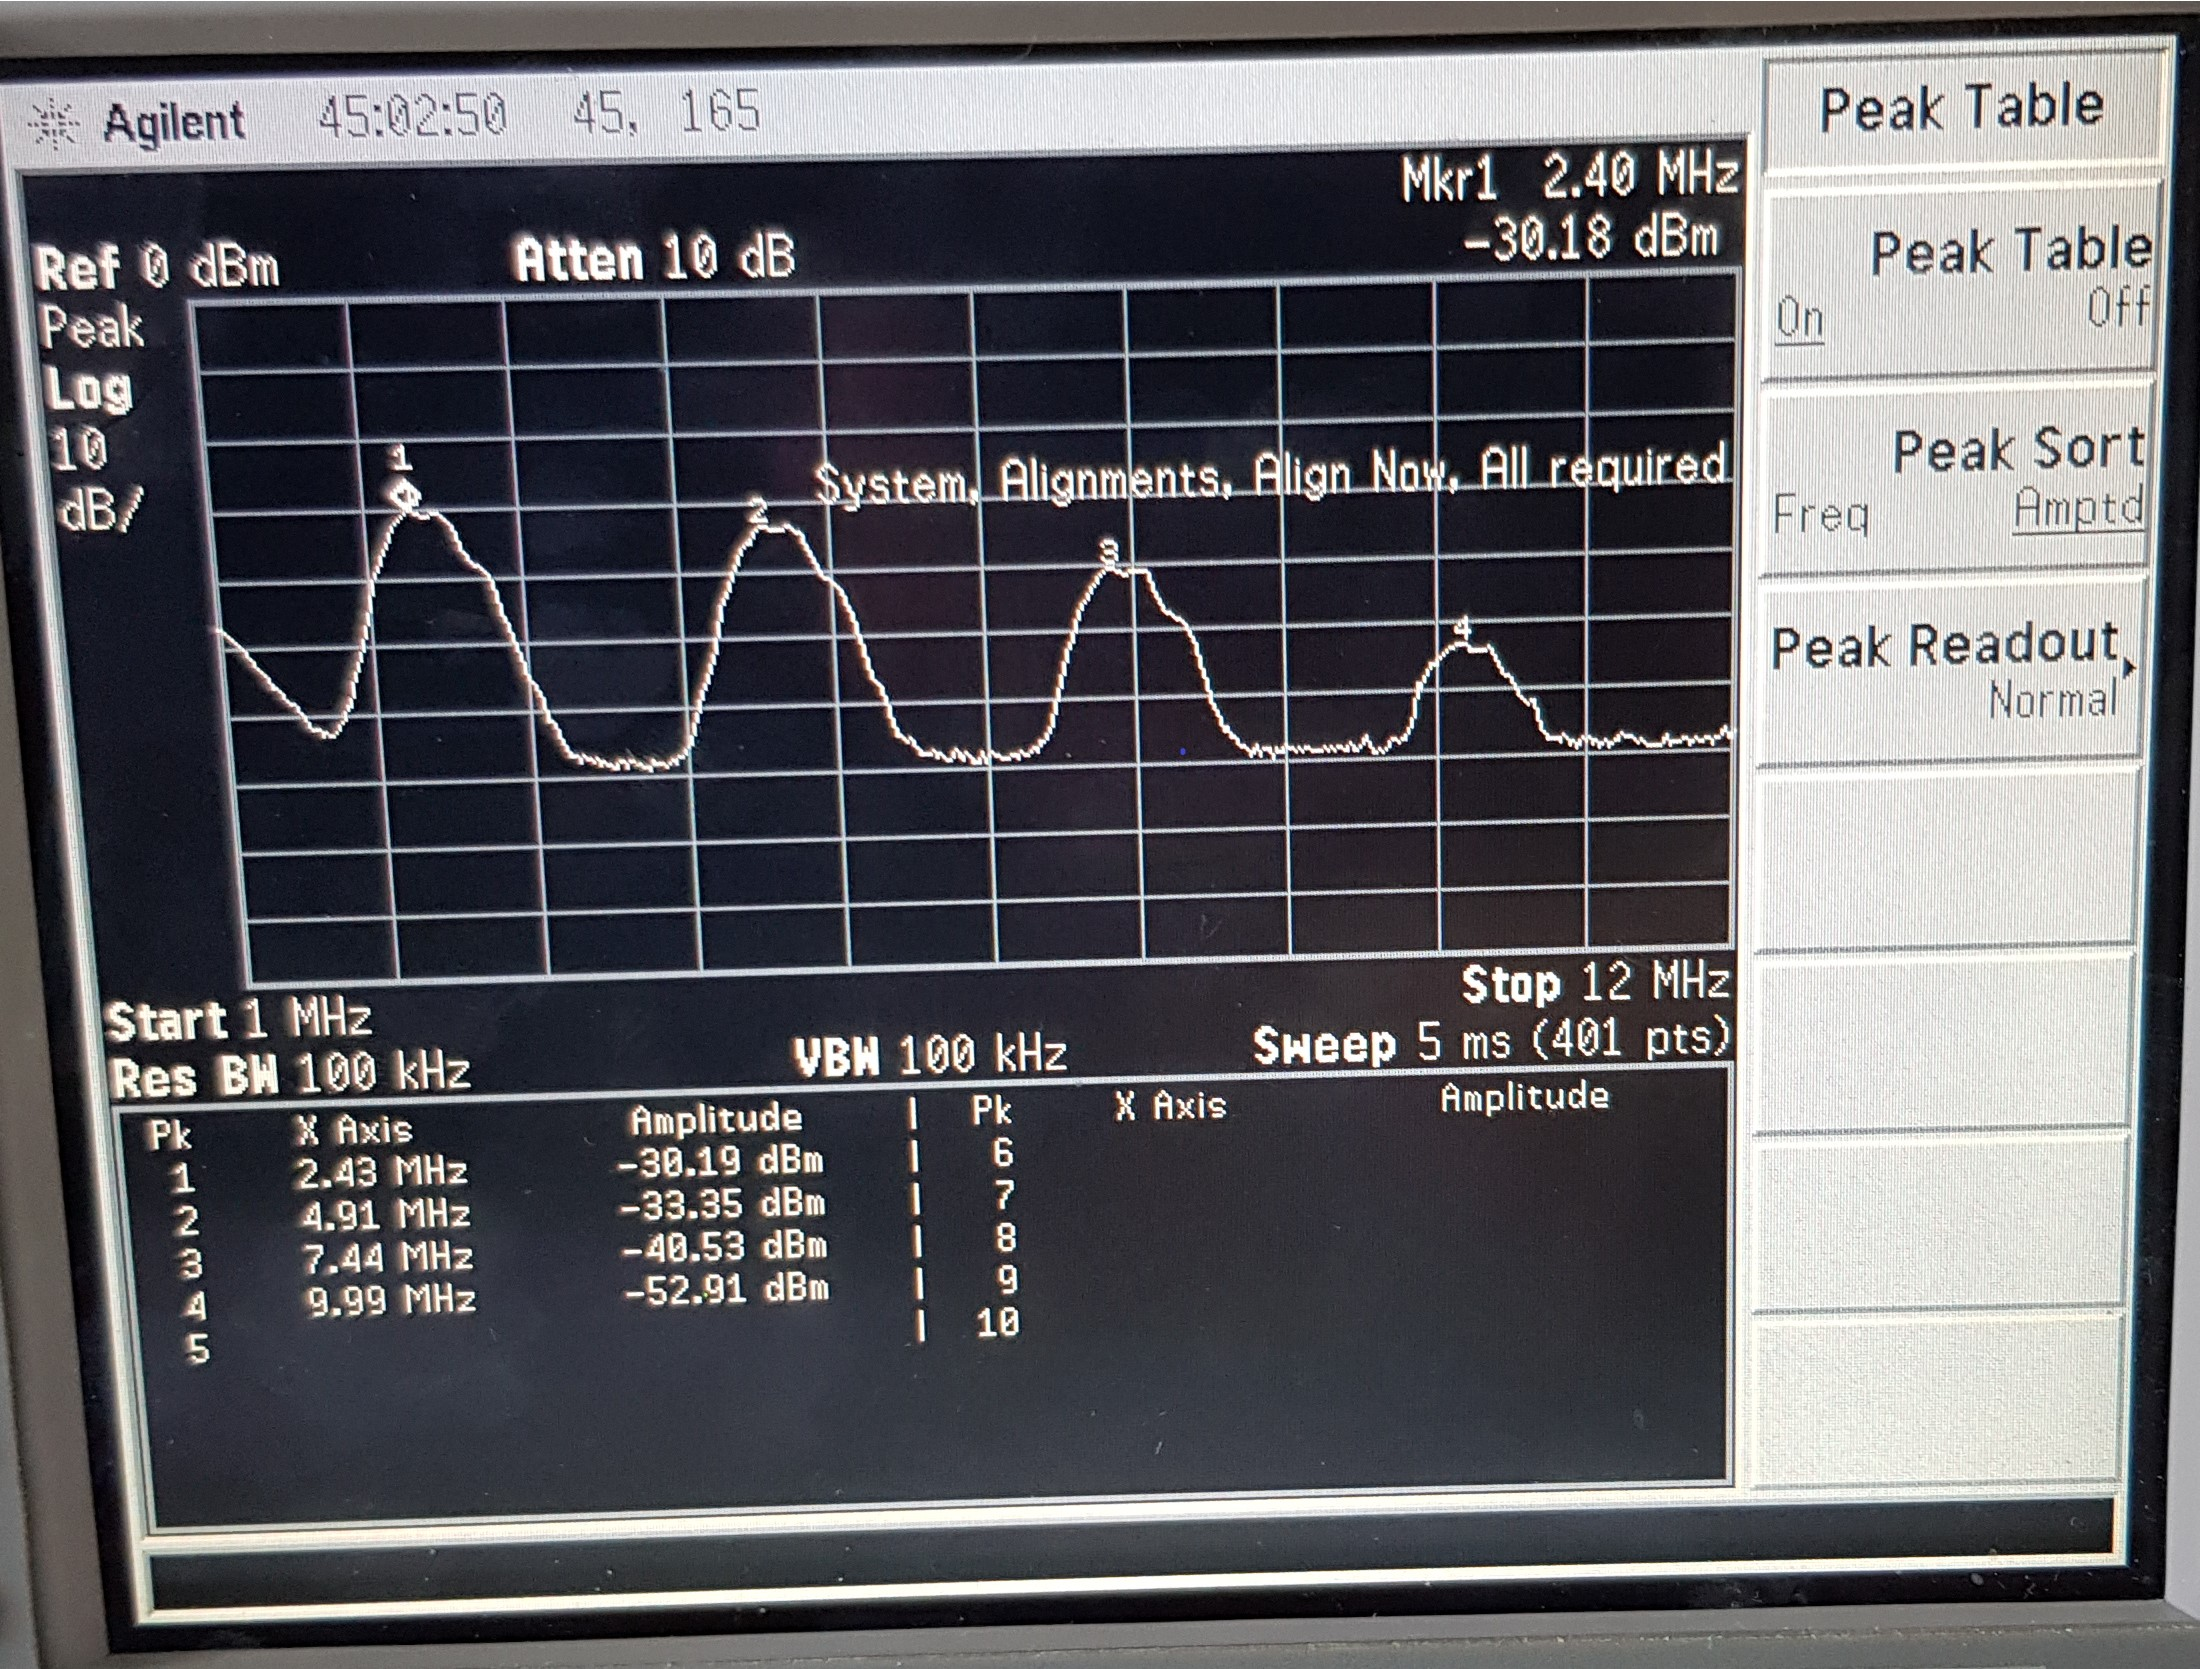
\includegraphics[width=0.7\textwidth]{spec/frequenzbereich_gross_diode.jpg}
  \caption{Amplitudenmodulierte
Schwingung einer Diode im Frequenzraum mit Oberschwingungen.}
\label{fig:diode_frequenz_gross}
\end{figure}




\subsubsection{(d) Erzeugen einer frequenzmodulierten Schwingung}
\label{subsubsec:auswertung_d}
Die Abbildung \ref{fig:freq_zeit} enthält eine zeitabhänige frequenzmodulierte
Schwingung, die durch die Schaltung aus Abbildung \ref{fig:15}
gebildet wird.
Da für die  $\SI{90}{\degree}$-Phasenverschiebung ein Laufzeitkabel mit der
Zeit T=$\SI{250}{\nano\second}$ verwendet wird, muss somit die
Trägerfrequenz gerade genau $f_{\text{T}}\SI{1}{\mega\hertz}$
betragen, um eine Phasenverschiebung um $\SI{90}{\degree}$
zu erzeugen. Als Modulationsfrequenz wird
$f_{\text{M}}=\SI{0.10(1)}{\mega\hertz}$ verwendet.

\begin{figure}
  \centering
  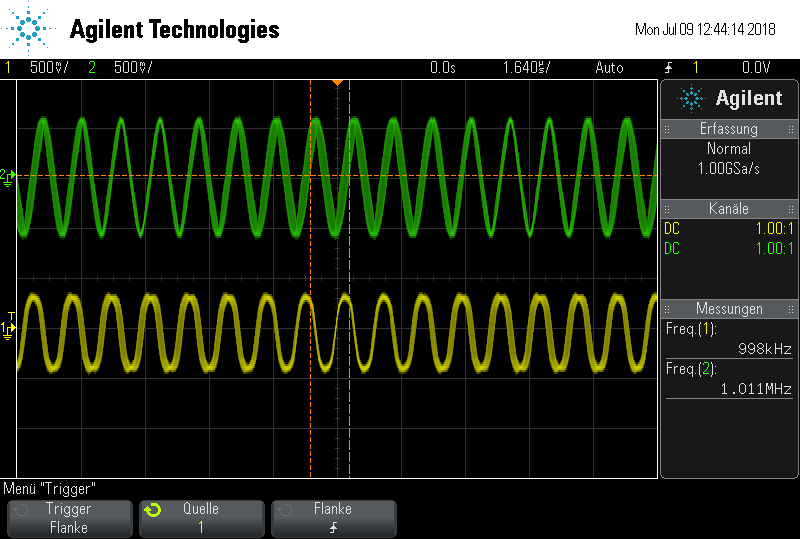
\includegraphics[width=0.7\textwidth]{osci/freq_mod.png}
  \caption{Trägerspammung ($U_{\text{T}}$ gelb) und Frequenzmodulierte
  Schwingung($U_3$ grün), die nach dem Aufbau aus Abb.\ref{fig:15} erzeugt wird.}
  \label{fig:freq_zeit}
\end{figure}
Der Modulationsgrad $m$ wird bei der Frequenzmodulation
aus der Verschmierung in x-Richtung des Signals bestimmt.
??
Die Abbildung \ref{fig:frequenz_freq} enthält die frequenzmodulierte Schwingung
im Frequenzraum.
\begin{figure}
  \centering
  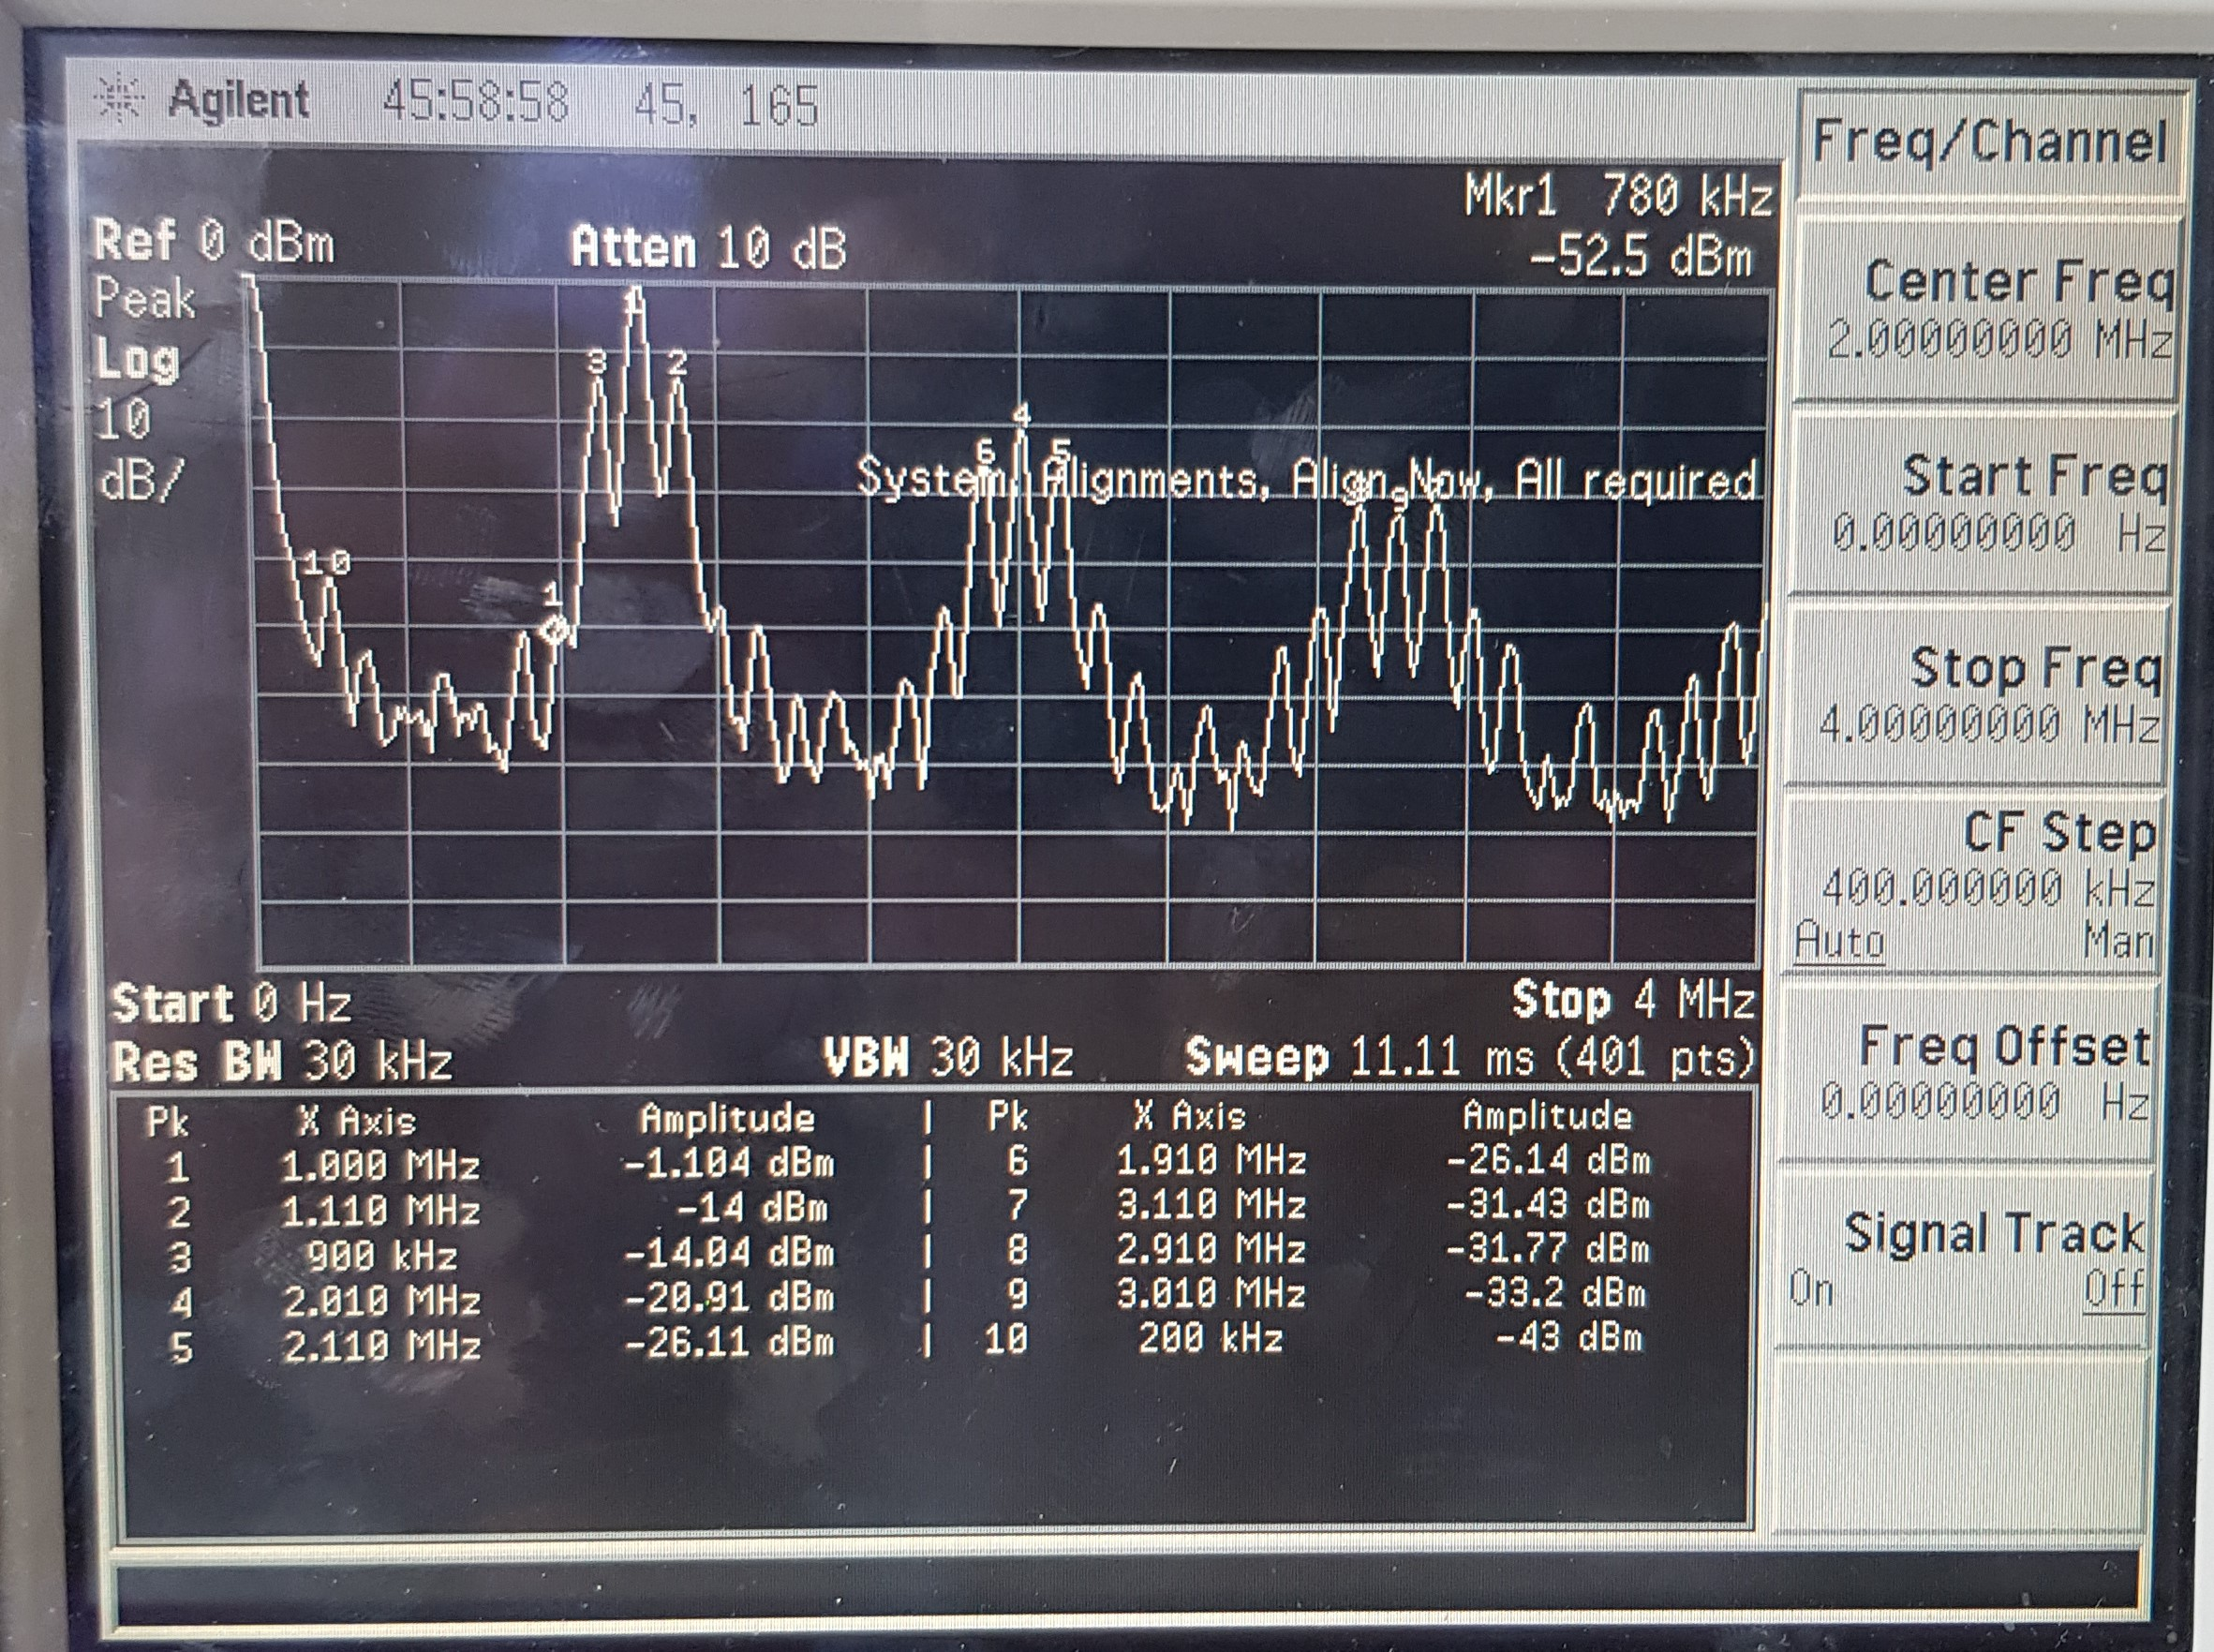
\includegraphics[width=0.7\textwidth]{spec/frequenzmodulation_bereich_fresh_cool.jpg}
  \caption{Frequenzmodulierte
Schwingung im Frequenzraum.}
\label{fig:frequenz_freq}
\end{figure}
Ebenfalls sind die Mischterme sowie die Trägerabstrahlung erkennbar.



\subsubsection{(e) Untersuchung der Phasenabhängigkeit eines
phasenempfindlichen Gleichrichters}
\label{subsubsec:auswertung_e}
Durch die Schaltung \ref{fig:15} wird ein phasenempfindlicher
Gleichrichter erzeugt. Um die Phase \phi zwischen
$\SI{0}{\degree}$ bis $\SI{360}{\degree}$ zu varieren, wird
auf Grund des Laufzeitkabel mit festem T=$\SI{250}{\nano\second}$
die Frequenz im Bereich von $\SI{1}{\mega\hertz}$-$\SI{5}{\mega\hertz}$
durchlaufen. Die Tablle \ref{tab:messwerte} enthält die gemessenen
Gleichspannungen $U_{\text{G}}$ für die entsprechende Phase $\phi$ und Frequenz $f$.
In der Abbildung \ref{fig:plot} ist die Gleichspannungen $U_{\text{G}}$
gegen die Phase aufgetragen.
\begin{table}
  \centering
  \caption{Messwerte der Gleichspannungen $U_{\text{G}}$, Phase \phi und Frequenz.}
  \label{tab:messwerte}
\begin{tabular}{c c c|}
\toprule
$f/\si{\mega\hertz}$ & $\phi / \si{\degree}$ &$ U_{\text{G}}/ \si{\milli\volt}$ \\
  \midrule
   1.0	&	90.0	&	13.0   \\
   1.2	&	108.0	&	34.7   \\
   1.4	&	126.0	&	50.7   \\
   1.6	&	144.0	&	60.0   \\
   1.8	&	162.0	&	67.0   \\
   2.0	&	180.0	&	69.1   \\
   2.2	&	198.0	&	61.7   \\
\bottomrule
\end{tabular}
\begin{tabular}{|c c c|}
  \toprule
  $f/\si{\mega\hertz}$ & $\phi / \si{\degree}$ &$ U_{\text{G}}/ \si{\milli\volt}$ \\
    \midrule
   2.4	&	216.0	&	45.3   \\
   2.6	&	234.0	&	21.2   \\
   2.8	&	252.0	&	2.1   \\
   3.0	&	270.0	&	-18.8   \\
   3.2	&	288.0	&	-36.5   \\
   3.4	&	306.0	&	-50.9   \\
   3.6	&	324.0	&	-60.3   \\
   \bottomrule
   \end{tabular}
  \begin{tabular}{|c c c}
    \toprule
    $f/\si{\mega\hertz}$ & $\phi / \si{\degree}$& $ U_{\text{G}}/ \si{\milli\volt}$ \\
      \midrule
   3.8	&	342.0	&	-64.4   \\
   4.0	&	0.0	&	-65.5   \\
   4.2	&	18.0	&	-58.0   \\
   4.4	&	36.0	&	-43.2   \\
   4.6	&	54.0	&	-21.0   \\
   4.8	&	72.0	&	0.5   \\
   5.0	&	90.0	&	21.9   \\
\bottomrule
\end{tabular}
\end{table}


\begin{figure}
  \centering
  \includegraphics[width=0.7\textwidth]{build/plot.pdf}
  \caption{Amplitude in Abhängigkeit von der Phase.}
  \label{fig:plot}
\end{figure}

\subsubsection{(f) Demodulation einer amplitudenmodulierten Schwingung
mit Hilfe eines Ringmodulators}
\label{subsubsec:auswertung_f}

\begin{figure}
  \centering
  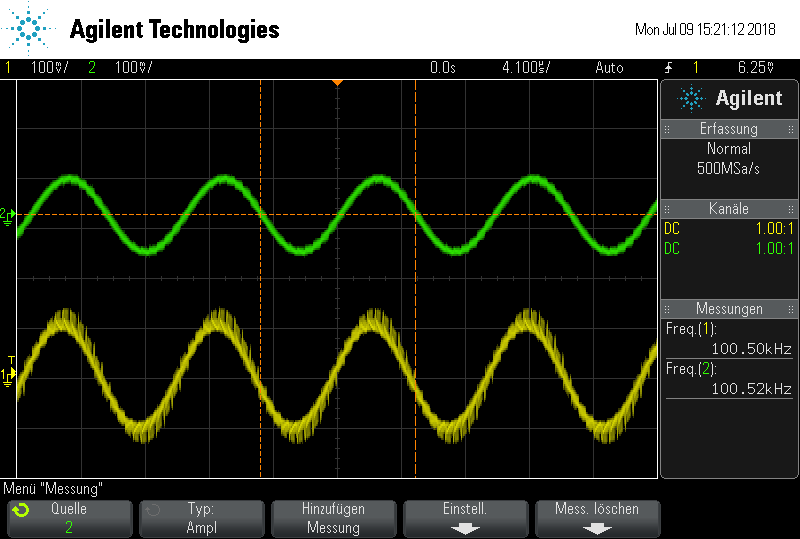
\includegraphics[width=0.7\textwidth]{osci/amp_demod.png}
  \caption{Demodulation von amplitudenmoduliertem Signal mit Hilfe eines
  Ringmodulator nach Schaltung \ref{fig:7}.}
  \label{fig:amp_demod_ring}
\end{figure}




\subsubsection{(g) Demodulation einer amplitudenmodulierten Schwingung
mit Hilfe einer Gleichrichterdiode}
\label{subsubsec:auswertung_g}

\begin{figure}
  \centering
  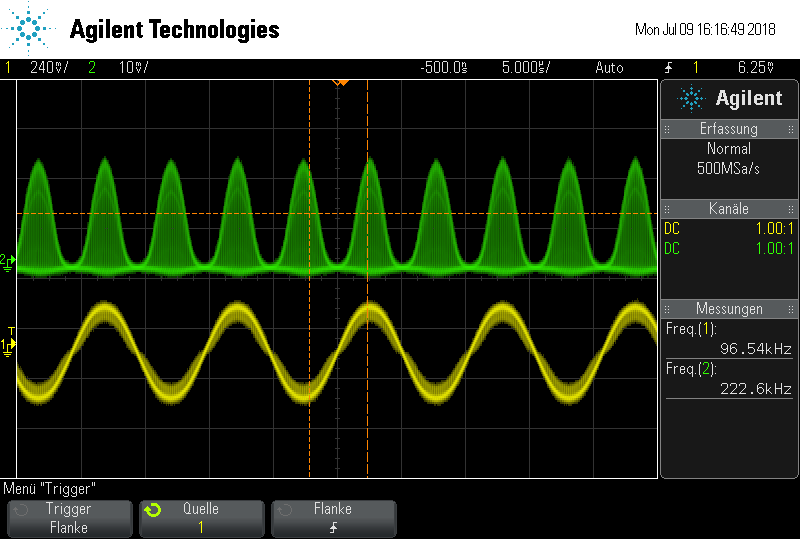
\includegraphics[width=0.7\textwidth]{osci/amp_demod_diode_A.png}
  \caption{Signal am Punkt A bei der Demodulation von amplitudenmoduliertem Signal mit Hilfe einer
  Diode und einem Tiefpass nach Schaltung \ref{fig:8}.}
  \label{fig:diode_punkt_A}
\end{figure}


\begin{figure}
  \centering
  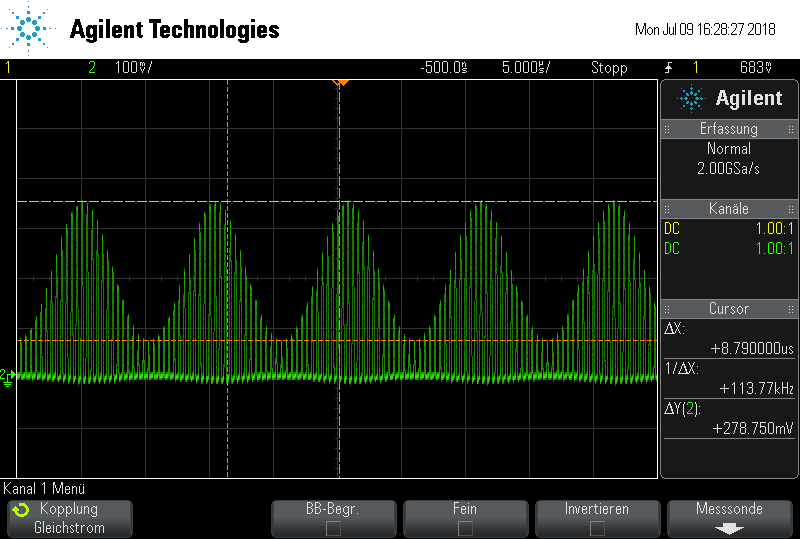
\includegraphics[width=0.7\textwidth]{osci/amp_demod_diode.png}
  \caption{Demoduliertes Signal von einem amplitudenmoduliertem Signal mit Hilfe einer
  Diode und einem Tiefpass nach Schaltung \ref{fig:8}.}
  \label{fig:diode_demod_amp}
\end{figure}



\subsubsection{(h) Demoduolation einer frequenzmodulierten Schwingung
mit Hilfe eines Flankendemodulators}
\label{subsubsec:auswertung_h}

\begin{figure}
  \centering
  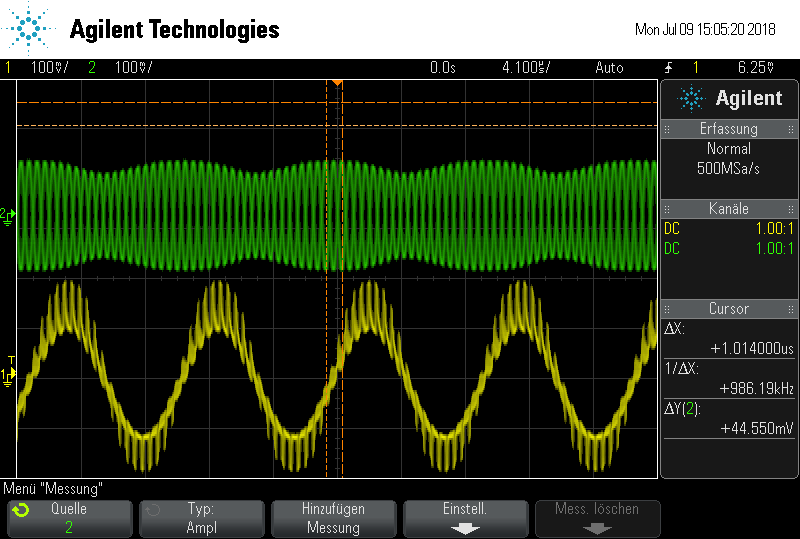
\includegraphics[width=0.7\textwidth]{osci/freq_demod_amp.png}
  \caption{Umwandelung eines Frequenzmodulierten Signales in ein Amplitudenmoduliertes
Signal mit durch einen Schwingkreis nach Abbildung \ref{fig:11}.}
\label{fig:freq_zu_amp}
\end{figure}



\begin{figure}
  \centering
  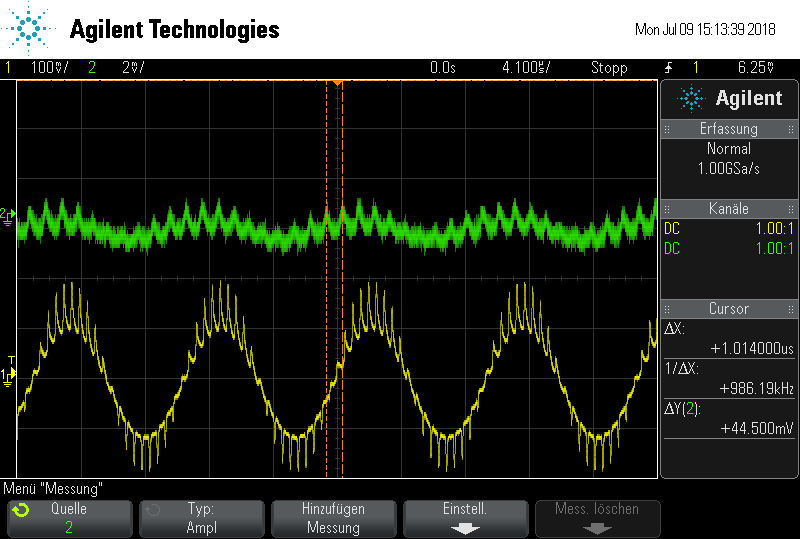
\includegraphics[width=0.7\textwidth]{osci/freq_demod.png}
  \caption{Demodulierung eines frequenzmodulierten Signales
  mit der Schaltung \ref{fig:11}.}
\label{fig:demod_frequenz}
\end{figure}
